\documentclass{article}
%% maxwidth is the original width if it is less than linewidth
%% otherwise use linewidth (to make sure the graphics do not exceed the margin)
\usepackage{natbib}
\usepackage{graphicx}
\usepackage{color}
\usepackage{enumerate}
\usepackage{hyperref}
\usepackage{tipa}
\usepackage{multirow}
\usepackage{times}
\usepackage{natbib}
\title{Perception and Production of Phonetic Change in York, Northern England: Update}
\begin{document}
\maketitle
\section*{Revisiting the aims of the PhD}

Sociolinguistic work over the past 40 years has yielded two key advances in the understanding of language variation and change. The first of these is a set of descriptive generalizations regarding the relationship between vocalic changes, or `principles' of vowel shifting (Labov, 1994:116). While variationist work has generally avoided questions of the cognitive or physiological basis of Labov's principles, a considerable body of evidence exists supporting their descriptive adequacy (e.g. Baranowski, 2008; Fridland \& Barlett, 2006). 

A second important strand of research is the development of more sophisticated approaches to understanding the way that social evaluations attach to linguistic variation, with the observation that variation plays a role in a complex social-semiotic system. Variable linguistic features may become associated with any number of locally-relevant social identities or personae; and may be drawn on in interaction as speakers align themselves toward or away from those social meanings (e.g. Eckert, 2000; 2008; Johnstone \& Kiesling, 2008; Zhang, 2008).  

While both of these strands of research provide important insights into mechanisms of language variation and change, less work has explicitly considered how systemic pressures and social pressures may interact in explaining the outcome of a sound change, particularly in British varieties of English. This thesis addresses this gap by by  comparing the predictions of an account of sound change dependent entirely on systemic pressures with one where the social meaning of the changing forms plays a role.

The present study builds on recent work conducted by Haddican et al. (2013) on \textsc{face/goat} diphthongization and \textsc{goose/goat} fronting in York, Northern England. The relationship between these changes allows predictions to be made regarding speakers' adoption of innovative forms. \textsc{face} and \textsc{goat} tend to diphthongize together in Northern Englishes, suggesting a process which targets phonological features rather than individual vowels (Watt, 2000; Haddican et al., 2013). Labov's `Principle III' predicts that \textsc{goose} fronting will be accompanied by (or followed by) the fronting of \textsc{goat}. Based on these generalizations alone, it would be predicted that speakers who participate in \textsc{face} diphthongization will also participate in \textsc{goat} diphthongization, and that speakers who participate in \textsc{goose} fronting will also be likely to participate in \textsc{goat} fronting. 

An account of linguistic change where speakers' identity plays a role would predict that individuals' social evaluation of the competing variants would influence their participation in or resistance to ongoing change. In this thesis it is argued that the best evidence for the role of social indexicality in sound change would come from a comparison of listeners' real-time evaluative reactions to the changing forms alongside data on their production patterns. This is achieved by first exploring evidence of the social meanings associated with the variable forms in this community using data from group interviews, then verifying speakers' intuitions through a perceptual experiment which quantifies the extent to which listeners' associate each variable with those meanings. 

Drawing on combined evidence from perception and production, the following hypotheses are tested:
\begin{enumerate}[(a)]
\item{Changes vary in the extent to which they participate in the local social-semiotic system.}
\item{Those changes which are less important socially are more widely adopted by members of the speech community.}
\item{While systemic pressures may explain the outcomes of change for some speakers, those speakers who strongly associate an innovative variant with stigmatized social meaning are likely to resist the ongoing change.}
\end{enumerate}
\newpage
\subsection*{\textsc{FACE/GOAT} diphthongization and \textsc{GOOSE/GOAT} fronting in York}
Haddican et al. (2013) report on a set of changes-in-progress in York -- \textsc{face}/\textsc{goat} diphthongization and \textsc{goose}/\textsc{goat} fronting\footnote{I think \textsc{goose} is also unrounding -- not discussed in detail by Haddican et al. (2013), but definitely need to think about this}. Comparing the speech of three age groups, the authors report that the fronting of \textsc{goose} is proceeding more quickly than \textsc{face}/\textsc{goat} diphthongization. 

The figure below is adapted from the figures on p.379 and p.389 of Haddican et al. (2013). The left-hand panel shows mean normalized Euclidean distances (measured at 10\% and 90\% of the vowel) for \textsc{face} and \textsc{goat}. The right-hand panel shows mean normalized F2 for \textsc{goose} and \textsc{goat} (measured at 70\% of the vowel for \textsc{goat} and 50\% of the vowel for \textsc{goose}; see Haddican et al. 2013 p.377 for more information). The letters represent three age groups: `O' referring to speakers born between and 1920 and 1939; `M' referring to speakers born between and 1967 and 1981, and `Y' referring to speakers born between 1987 and 1990. 

\begin{figure}[ht!]
\hspace{-1.5cm}
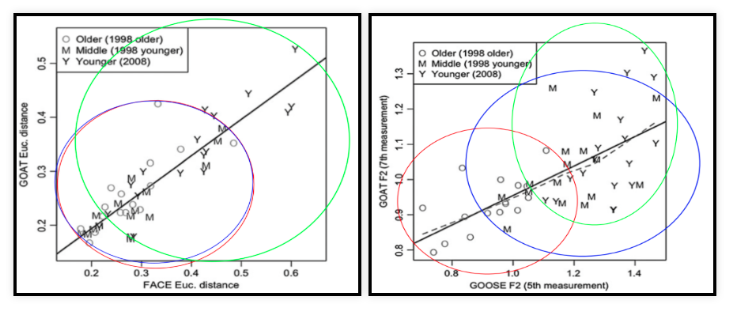
\includegraphics[scale=0.6]{D_lawrence_fronting_and_diphthongization.png}
\caption{Mean normalized Euclidean distances for \textsc{face} and \textsc{goat} (left) and mean normalized F2 values for \textsc{goose} and \textsc{goat} (right).}
\end{figure}

In order to highlight the authors' argument regarding the rates of change, I have added approximate minimum volume enclosing ellipsoids to the original figures. These are the smallest possible ellipsoids which can be drawn to enclose all members of a given age group, with red representing the oldest speakers, blue representing the middle group, and green representing the youngest group. The fact that the oldest (red) and middle (blue) speakers have near-identical ellipsoids for \textsc{face}/\textsc{goat} diphthongization demonstrates that there was very little change between those two generations. In contrast, the middle age group appears to pattern closer to the younger speakers with regard to \textsc{goose}/\textsc{goat} fronting. Haddican et al. (2013) interpret this as reflecting the rapid spread of \textsc{goose} fronting in comparison to the other changes.

The second observation that Haddican et al. (2013) make is that there is a correlation between the degree of \textsc{goat} diphthongization and \textsc{goat} fronting, and that the degree of this correlation varies between age groups, as shown in the figure below (from Haddican et al., 2013, p.390).

\begin{figure}[ht!]
\centering
\includegraphics[scale=0.6]{goat_correlation.png}
\caption{Correlation of mean normalized Euclidean distance and  mean normalized F2 for \textsc{goat}.}
\end{figure}

These data suggest that while there is some evidence of fronted, monophthongal variants among the `M' speakers, younger speakers appear to avoid these variants. Following Labov's (1994) generalizations regarding vowel shifts, it might be expected that \textsc{goat} would front along with \textsc{goose}. A complete lack of \textsc{goat} fronting could be treated as counter-evidence to Labov's generalizations. However, the available evidence suggests that the co-fronting of \textsc{goose} and \textsc{goat} does occur, but that some speakers (particularly young speakers who monophthongize \textsc{face} and \textsc{goat}) tend to resist it.  

Haddican et al. (2013) suggest that the different progression of the changes is related to their social evaluation. Their claims are as follows:

\begin{itemize}
\item{Monophthongal \textsc{face} \& \textsc{goat} are associated with local regional identity, leading to the diphthongization of these forms proceeding more slowly than the fronting of \textsc{goose}.}
\item{Fronted \textsc{goose} variants are not associated with any salient social meaning, facilitating their rapid adoption.}
\item{Fronted, monophthongal \textsc{goat} variants may be associated with a stigmatized, working-class subgroup, particularly amongst younger speakers, explaining variable co-fronting of \textsc{goose} and \textsc{goat}.}
\end{itemize}

Underpinning this argument are the following claims about how sound changes spread through a speech community:

\begin{enumerate}[i]

\item{\textbf{When a set of innovations enter a speech community, they attract different levels of social evaluation.} Some variants (such as monophthongal \textsc{\textsc{face}} and \textsc{\textsc{goat}}) may become indexical of particular social groups or characteristics, while other variants (such as fronted \textsc{\textsc{goose}}) may not attach to any salient social meaning.}
\item{\textbf{Variants which attract a strong social evaluation are likely to be adopted more slowly than those which attract little social evaluation.} In the case of changes whose variants do not attract a strong social evaluation, the innovation may spread rapidly. In the case of changes whose variants attract a strong social evaluation, adopting or resisting the change will have social consequences, meaning that the change is likely to spread less rapidly.}
\item{\textbf{The social indexicality of competing forms may inhibit systemic pressures in determining the outcome of sound change.} For example, if a stigmatized social meaning attaches to a form, speakers may resist change where it might otherwise be expected.}
\end{enumerate}

The evidence for the above arguments is as follows:

\begin{enumerate}[(a)]
\item{Production data from three age groups, showing the rapid uptake of \textsc{goose} fronting among speakers born post 1967 and shift toward diphthongal \textsc{face/goat} among speakers born post 1987.}
\item{Metalinguistic commentary elicited during ethnographic interviews. While \textsc{face} and \textsc{goat} monophthongs are both mentioned and imitated during discussions of York/Yorkshire dialect, fronting is not mentioned, except for one instance where a speaker uses a fronted monophthong in a performance of `chav' speech.}

\item{Correlations between speakers' scores on an 8-point attitudinal index and their production values -- the degree of \textsc{face}/\textsc{goat} diphthongization is shown to correlate with more positive attitudes to the local community; while this correlation is also true for \textsc{goat} fronting, it is much weaker for \textsc{goose} fronting.}

\end{enumerate}

Overall, the argument presented by Haddican et al. (2013) is highly compelling in its discussion of the relative contribution of social and linguistic pressures in explaining the outcome of sound change. However, the evidence presented has a number of limitations. 

With regard to point (a), there is a potential issue with sampling bias. Since no information is given regarding the socioeconomic status or social network structure of the informants, there is a strong possibility that the apparent jump toward diphthongal variants of \textsc{face} and \textsc{goat} represents sampling bias rather than actual change. From figure 1 it is clear that the intergroup difference is carried by a subgroup of four younger speakers, meaning that this is weak evidence of widespread change of any kind. 

With regard to the ethnographic interview data (b), there is an issue of treating the absence of evidence as evidence -- while speakers may not mention \textsc{goose} fronting in their metalinguistic discussions, this does not mean that \textsc{goose} variants do not attract a social evaluation of some sort. With regard to the single performed token of a fronted, monophthongal \textsc{goat} variant, there is no reason to think that the association between this form and `chav' speech is shared by other York speakers, nor that this association is particularly strong among younger speakers\footnote{Actually, the `chav' meaning is contested directly after the excerpt presented by Haddican et al. (2013), but the authors don't discuss this.}. 

The attitudinal index (c) is quantitatively unconvincing -- responses to the researchers' 8-point scale are heavily negatively skewed, and while the authors report \textit{p} values for regression models with a term derived from this index, no information is given about the amount of variance explained by this predictor. A further issue with this index is that it does not provide evidence of the social indexical significance of the variants themselves, nor the role of this significance in the outcome of linguistic change -- rather, it demonstrates that the same speakers who respond highly on an attitudinal scale are those who are likely to avoid linguistic innovations. %The general pattern of argument is a common one in sociolinguistic work -- identifying group-level linguistic variation correlated with a social characteristic (which could include gender, ethnicity, or responses to an attitudinal questionnaire), and treating this variation as reflecting the social-indexical properties of the variable form. 
\newpage
\subsection*{What would be the best possible evidence for the role of social indexicality in sound change as put forward by Haddican et al. (2013)?}

Returning to Haddican et al.'s (2013) argument, the following sources of evidence would provide better support:
\begin{enumerate}[i]
\item{\textbf{When a set of innovations enter a speech community, they attract different levels of social evaluation.}
\\Qualitative evidence of the types of social meanings associated with the competing forms of each change, and quantitative evidence that the different changes are linked to these meanings to different extents.}
\item{\textbf{Variants which attract a strong social evaluation are likely to be adopted more slowly than those which attract little social evaluation.} 
\\Evidence that those changes which are less strongly linked with social evaluations are more widely adopted in the community.}
\item{\textbf{The social indexicality of competing forms may inhibit systemic pressures in determining the outcome of sound change.} 
\\Evidence of linguistically expected shifting of vowels among some speakers (e.g diphthongization of both \textsc{face} and \textsc{goat}, or fronting of both \textsc{goose} and \textsc{goat}), but less so among those speakers who associate the innovative variant with a stigmatized social meaning.}
\end{enumerate}

%While the above points are not made fully explicit in their paper, they are hinted toward in the authors' mention of \textit{off the shelf} and \textit{under the counter} changes, terms originally introduced by Milroy (2007). Milroy (2007) defines an \textit{off the shelf} change as one which is `relatively freely available to appropriately positioned social actors as a stylistic and social resource, regardless of the structure and location of their primary social networks' (p.151), while an \textit{under the counter} change is one which `requires the repeated exposure provided by regular social interaction'. As discussed by Fridland (2008), the distinction is essentially one between \textit{local} and \textit{supralocal} changes. Summarizing Milroy's (2007) argument, the following distinctions are made:

%\begin{table}[!ht]
%\hspace{-1cm}
%\begin{tabular}{|p{3cm}|p{5cm}|p{5cm}|}
%\hline
 %                                       & Local changes                                          & Supralocal changes                                                                \\ \hline
 %Rate of change                          & Spread more slowly and in a less regular fashion       & Spread rapidly and in a regular fashion                                           \\ \hline
 %Network structure                       & Constrained by network structure                       & Available to all speakers -- network structure less important                     \\ \hline
 %Social-indexical properties             & Strongly linked to local social meanings               & No strong social evaluation                                                       \\ \hline
 %Linguistic conditioning                 & Complex linguistic conditioning may be maintained      & Complex linguistic conditioning unlikely due to lack of regular face-to-face interaction                                         \\ \hline
 %Role of cognitive/physiological factors & Change constrainted by cognitive/physiological factors, but the social embedding of the variants may interfere with these & Change driven by cognitive/physiological factors, with little social interference \\ \hline
 %\end{tabular}
 %end{table}

%\newpage

%The distinction between \textit{off the shelf} and \textit{under the counter} changes provides a testable prediction regarding the role of social indexicality in constraining linguistic change -- it predicts that changes whose variants play an important sociolinguistic role in the speech community are likely to be adopted more slowly than changes with a less salient social anchoring. 

%The following evidence is provided by Haddican et al. (2013) to support their claim that FACE/GOAT diphthongization and GOAT fronting constitute 5'under the counter' changes while GOOSE fronting is an 'off the shelf' change:
%\begin{enumerate}[i]
%\item{\textbf{Rate/regularity of change}

%The authors demonstrate that the fronting of GOOSE is more widespread than the other changes. The fact that the 'M' group pattern with the 'Y' group with regard to this change is interpreted as reflecting its rapid spread; in contrast, FACE and GOAT are diphtongized more markedly among the 'Y' group, while the 'M' and 'O' groups pattern together.}

%\item{\textbf{Linguistic conditioning}

%In York, GOOSE fronting occurs across the formant trajectory and not principally in the nucleus (as reported in US varieties by e.g. Baranowski, 2008; Hall-Lew, 2004). This is interpreted as evidence of the linguistic conditioning on a change varying across speech communities, aligning with point (iii) in the table above. In addition, there is evidence of an effect of following voicing on FACE diphthongization, where following voiceless consonants favour longer Euclidean distances. This could be interpreted as evidence of the sort of phonological conditioning expected in 'under the counter' changes.}

%\item{\textbf{Role of cognitive/physiological factors}

%These factors are not discussed in detail by Haddican et al. (2013), except for the reference to Labov's (1994) Principle III of chain shifts. However, back vowel fronting is well attested in other varieties (...), with arguments such as (x, y, z) suggesting a role of cognitive and physiological factors in its spread. In contrast, there are no published sources providing a similar account of diphthongization.
%}

%\item{\textbf{Social-indexical properties}

%The main source of evidence comes from metalinguistic commentary elicited during ethnographic interviews. While FACE and GOAT monophthongs are both mentioned and imitated during discussions of York/Yorkshire dialect, fronting is not mentioned, except for one instance where a speaker uses a fronted monophthong in a performance of 'chav' speech. 

%A second source of evidence for the social-indexical properties of the variants comes from correlations between speakers' scores on an 8-point attitudinal index -- the degree of FACE/GOAT diphthongization is shown to correlate with more positive attitudes to the local community, while this correlation is also true for GOAT fronting, it is much weaker for GOOSE fronting.

%Finally, there is limited evidence in the form of stylistic variation, operationalized by contrasting interview speech with word list productions. Diphthongal variants of FACE are preferred in read speech, with a non-significant trend in the same direction for GOAT. No significant stylistic effects on GOAT fronting are found, and no evidence is presented regarding any stylistic constraints on GOOSE fronting.

%}

%\item{\textbf{Network structure}

%No evidence is presented regarding network structure, nor any other independent speaker variable (such as socioeconomic status).
%}
%\end{enumerate}

\newpage

\section*{Group interviews}

During the first stage of data collection, I conducted a series of small group interviews with a sample of York residents. The aim of these was to find out:

\begin{enumerate}[(a)]
\item{Which (if any) social groups / meanings do York speakers associate with the competing variants of the changing forms?}
\item{What other socially-meaningful practices are associated with the groups / meanings identified above?}
\end{enumerate}

Addressing these two questions is essential to testing the central claims of Haddican et al. (2013). In their ethnographic data, the authors provide present evidence from speakers' metalinguistic commentary that the forms have the following social meanings:

\begin{itemize}
\item{monophthongal \textsc{face}/\textsc{goat} are associated with local identity -- described as `typical York/Yorkshire'.}
\item{Fronted, monophthongal \textsc{goat} is associated with a stigmatized `chav' subgroup.}
\item{Fronted \textsc{goose} carries no consistent social evaluation.}
\end{itemize}

%Sub-question (a) above aimed to collect further qualitative evidence with regard to these claims. The motivation for sub-question (b) was to inform the design of the subsequent perception test. Much previous socio-perceptual work has used various kinds of rating scale based around standard demographic categories or standardized evaluation scales. However, these approaches are limited in that they rely on the researcher deciding \textit{a prioi} on the form and content of the elicitation scales. Any perceptual task eliciting social evaluations would benefit from being based on concepts relevant to the population under study. Thus, sub-question (b) aimed to elicit from participants the clusters of social practices (such as forms of dress, consumption choices, meeting places) associated with the relevant social groups, which could then be integrated into the perception test.

The approach adopted in the group interviews was based on Campbell-Kibler (2007), who investigated the social meaning of variation in (ing) among US university students. To do this, the author conducted a set of group interviews where participants listened to recordings of speakers using velar or apical `ing' and were asked to comment on their impressions of each speaker. The reactions collected in this way informed the construction of a perceptual survey, which allowed the consistency and strength of listeners' intuitions to be measured. In the present study, participants heard a range of York speakers of different ages and backgrounds using the variants under study, and were asked to discuss their impression of those speakers. 

\newpage
\subsection*{Selecting stimuli for group interviews}

Speech stimuli for the group interviews were extracted from existing corpora of York speech -- recordings of 47 speakers made in 1997 as part of Tagliamonte's (1998) \textit{Roots of Identity} project, and 18 speakers recorded in 2008 as part of Haddican's (2014) \textit{A Comparative Study of Language Change in Northern Englishes} project. These data consisted of a set of audio files and text transcriptions. In order to facilitate the selection of stimuli, my first step was to generate time-alignments of the recordings and transcriptions. This allowed me to quickly find examples of conservative and advanced productions of the changing variables.

\subsubsection*{Indexing the York corpora}

The Tagliamonte (1998) and Haddican (2013) data consist of a set of hour-long audio files accompanied by text transcriptions marked with minute intervals. In order to quickly generate a searchable corpus of these files, I generated time-alignments using the University of Penn FAVE (Forced Alignment and Vowel Extraction) toolkit (Rosenfelder et. al, 2011). This program performs \textit{forced alignment} of text to speech. Given a speech sample and short transcription, the program attempts to identify the start and end points of each transcribed word in the recorded speech. It does this by first consulting a list of stored phone-level transcriptions of words (the `dictionary'), then comparing spectral characteristics of the speech sample to a set of phone models generated from human-annotated training data. In this way, the program finds the best possible alignment of each text transcription for the audio provided.


I wrote a script in \textit{R} which converted the text files into tab-delimited files suitable for forced alignment. The main function of this script was to identify each minute-long segment of each the transcription (based on the transcribed minute intervals), then add it to a table with start and end times in seconds. In addition, the script removed any annotation comments and timed pauses (which would be interpreted by the aligner as transcribed speech). The script then formatted the transcription text as specified in the FAVE transcription guidelines (\url{http://fave.ling.upenn.edu/downloads/Transcription_guidelines_FAAV.pdf}). Finally, the script searched the text transcription for biographical information from each participant and passed this to a speaker file, which is required by the FAVE system. This process iterated over the entire set of 100 transcriptions, passing the converted files to the FAVE aligner automatically from within \textit{R}. Since the dictionary file used by FAVE is based on the CMU pronouncing dictionary, I created a custom dictionary for the York recordings and added transcriptions where necessary.

The result of running this script on the York data was a set of TextGrid files, providing time-aligned word-level transcriptions of the interviews. I evaluated a 30s sample of each recording by comparing the transcription with the audio in \textit{Praat} -- while word-level transcriptions are highly accurate, there are two limitations:

\begin{itemize}
\item{The TextGrids make no distinction between individual speakers.}
\item{There are errors in the phone-level transcription, probably due to the fact that the FAVE aligner was trained on US English data.}
\end{itemize}

Automatic measurements were conducted with the \textit{FAVE-extract} program, resulting in a table of estimated formant values at five measurement points for each vowel token identified, as well as information about the host word, preceding and following linguistic context, and start and end times. By importing this table into \textit{R} it was possible to search for tokens based on arbitrary criteria; using the \textit{PraatR} package (Albin, 2014), it was possible to quickly browse the entire set of recordings and play excerpts, facilitating the quick selection of stimuli.

\subsubsection*{Selecting stimuli}
 14 extracts were selected from the resulting time-aligned corpus. These were selected to provide examples of the changing variables, spoken by speakers of a range of ages. In order to narrow down the candidate excerpts, I searched for the most frequent lexical items containing each variable (excluding function words), and selected excerpts containing those words. As well as improving the efficiency of finding appropriate samples, keeping the target lexical item constant across samples facilitated discussion in the group interviews -- it was possible to draw participant's attention to the pronunciation of lexical items, rather then having to discuss the pronunciation of the variable in a more abstract sense. The lexical items used are summarized below:

\begin{table}[h]
\centering
\begin{tabular}{|l|l|lll}
\cline{1-2}
Variable & Lexical item                  &  &  &  \\ \cline{1-2}
\textsc{face}     & \textit{ages}                       &  &  &  \\ \cline{1-2}
\textsc{goat}     & \textit{road}                        &  &  &  \\ \cline{1-2}
\textsc{goose}    & \textit{food}                       &  &  &  \\ \cline{1-2}
\end{tabular}
\end{table}
After extracting all instances of each of these words from the corpus, I listened through them in order to identify excerpts containing clearly-audible instances of each variant. After identifying a clearly-audible token of a target variant, I extracted preceding and following material to situate the token in a clear conversational context, usually from the beginning to the end of the utterance. The length of the extracts ranged from 8.9s to 33s, with a mean length of 21.6s. 

The table below summarizes the recordings selected:
\newpage
\begin{table}[!ht]
\centering
\begin{tabular}{|l|l|l|l|l|}
\cline{1-5}
Stimulus no. &Variable&Variant&Speaker&Extract\\
\cline{1-5}
1&\textsc{face}&\textipa{[e:]}&M,74&\parbox{5cm}{\vspace{.25\baselineskip}...we could'a gone on for \textbf{ages}, it was just nicely warmed up, the to-in' and fro-in' and questions and answers; it were \textbf{great.}\vspace{.25\baselineskip}}\\
\cline{1-5}
2&\textsc{face}&\textipa{[eI]}&F,80&\parbox{5cm}{\vspace{.25\baselineskip}...for quite a while afterwards I had dizzy \textbf{headaches}; I used to get into bed and the whole room was going around, and I had to be very careful not to knock my head or anything for \textbf{ages}.\vspace{.25\baselineskip}}\\
\cline{1-5}
3&\textsc{face}&\textipa{[e:]}&F,40&\parbox{5cm}{\vspace{.25\baselineskip}...so she was there with me for \textbf{ages}, then she went home; I still had my contact lenses in, aye, I was wearing my contact lenses, and they were all going `I'm \textbf{amazed} they're still in!'\vspace{.25\baselineskip}}\\
\cline{1-5}
4&\textsc{face}&\textipa{[eI]}&F,19&\parbox{5cm}{\vspace{.25\baselineskip}...when does she not talk for \textbf{ages}? Just `I can't stop! I can't stop!' and then an hour \textbf{later} she leaves.\vspace{.25\baselineskip}}\\
\cline{1-5}
5&\textsc{goat}&\textipa{[o:]}&M,55&\parbox{5cm}{\vspace{.25\baselineskip}...I went out on t'main \textbf{road}, \textbf{over} this bridge; then he said well if you \textbf{don't} mind I'll have a \textbf{go}, I said I \textbf{don't} mind it's your wagon you \textbf{own} it...\vspace{.25\baselineskip}}\\
\cline{1-5}
6&\textsc{goat}&\textipa{[\textschwa\textipa{U}]}&F,56&\parbox{5cm}{\vspace{.25\baselineskip}...because she lives up Tranby avenue which is off Hull \textbf{Road}, and poor Jonothan \textbf{goes} to Badger Hill school. so if he went to Heslington Sunday School he'd be meeting children he \textbf{knows}.\vspace{.25\baselineskip}}\\
\cline{1-5}
7&\textsc{goat}&\textipa{[o:]}&F,35&\parbox{5cm}{\vspace{.25\baselineskip}...and there you can't cross \textbf{over} the street by car 'cos there's like barriers. We had to \textbf{go} right past the \textbf{hotel} to the end of the \textbf{road} and then come back on their side.\vspace{.25\baselineskip}}\\
\cline{1-5}
\end{tabular}
\end{table}

\begin{table}[!ht]
\centering
\begin{tabular}{|l|l|l|l|l|}
\cline{1-5}
Stimulus no.&Variable&Variant&Speaker&Excerpt\\
\cline{1-5}
8&\textsc{goat}&\textipa{[oU]}&M,20&\parbox{5cm}{\vspace{.25\baselineskip}I've never been knocked off my bike. Erm, I've had an accident on my bike \textbf{going} \textbf{over} Lendal Bridge. They were resurfacing it and it was night and there was just this huge \textbf{hole} in the \textbf{road} that they hadn't marked out. They'd taken all the surface off and not put any bollards out, probably because they'd all been \textbf{stolen.}\vspace{.25\baselineskip}}\\
\cline{1-5}
9&\textsc{goat}&\textipa{[8]}&F,43&\parbox{5cm}{\vspace{.25\baselineskip}...and that traffic can be queued back beyond Knavesmire \textbf{Road}, which never used to happen. \textbf{So} I dive off down Knavesmire \textbf{Road} now, an' round at Bishopthorpe \textbf{Road}, which is just creatin' more traffic on another \textbf{road}! \vspace{.25\baselineskip}}\\
\cline{1-5}
10&\textsc{goat}&\textipa{[\textschwa U]}&F,20&\parbox{5cm}{\vspace{.25\baselineskip}...you would think that if they want less people on the \textbf{road} then they would make the bus free...\vspace{.25\baselineskip}}\\
\cline{1-5}
11&\textsc{goose}&\textipa{[u:]}&F,80&\parbox{5cm}{\vspace{.25\baselineskip}...aye, he'd gone thinner an' all that; they didn't get the proper \textbf{food} like. They lived on corned beef an' all that\vspace{.25\baselineskip}}\\
\cline{1-5}
12&\textsc{goose}&\textipa{[u:]}&F,20&\parbox{5cm}{\vspace{.25\baselineskip}...they worked four hours in the morning and they got their accommodation and \textbf{food} and \textbf{use} of the sports facilities, so it was alright...\vspace{.25\baselineskip}}\\
\cline{1-5}
13&\textsc{goose}&\textipa{[0:]}&F,35&\parbox{5cm}{\vspace{.25\baselineskip}...and I remember there was a strawberry patch. Trust me to remember the \textbf{food.}\vspace{.25\baselineskip}}\\
\cline{1-5}
14&\textsc{goose}&\textipa{[0:]}&F,20&\parbox{5cm}{\vspace{.25\baselineskip}...it was very nice \textbf{food}. I can't remember what it was but it was very nice.\vspace{.25\baselineskip}}\\
\cline{1-5}
\end{tabular}
\end{table}

\newpage

These extracts were chosen not only to include examples of the variants of interest, but also to be representative of speakers of a range of ages and genders. The motivation for this was to stimulate discussion on the social groups and practices relevant to York speakers.

 While the three changing vowels are the focus of this study, the aim of the group interviews was to elicit as much information as possible on aspects of the informants' social world relevant to language use. In addition to the target variants, the recordings contain a number of features which are reported to be sociolinguistically important -- for example, was/were variation in item 1 and definite article reduction in item 5. While the presence of these features would be problematic in a controlled experiment, their presence in an open elicitation task is less of a problem -- the aim of this task was to uncover the styles and personae which are relevant to the informants' social and linguistic practice. The perspective adopted for this phase of data collection was that a range of linguistic variables are likely to be associated with those styles or personae, rendering the presence of non-focal features unproblematic. Construing sociolinguistic meaning as constituted of a set of social concepts which are associated with groups of linguistic variables, the aim of the interviews was to uncover those concepts, while the aim of the perceptual experiment was to quantify relative association between the changing vowels and the previously-identified social schemata.

During piloting of the stimuli among colleagues it was pointed out that some recordings were of noticeably higher quality than others. This is likely due to the fact that Tagliamonte's (1997) recordings were conducted with lower-fidelity equipment than those of Haddican (2014). In an attempt to avoid listeners' attention being drawn to the difference in recording quality, the more recent recordings were downsampled to match the sampling frequency of the older recordings (22050Hz) , and all stimuli were low-pass filtered to 5000Hz. The resulting recordings were judged clearly audible by the author, and at no point did any of the participants comment on the quality of the samples.


\newpage
\subsubsection*{Group interview recruitment}

During the recruitment of focus group participants, a strong emphasis was made on identifying individuals who were representative of as broad a range of York speakers as possible. The following methods of recruitment were used:

\begin{itemize}
\item{Word-of-mouth recruitment through colleagues at the University of York (3 participants).}
\item{An advertisement on a Facebook group called `Things for Sale or Swap in York', primarily used by people with lower incomes to exchange household goods (2 participants).}
\item{An advertisement on a Facebook group called `Tree of Jobs in York', primarily used by young people looking for work in manual or service industries (3 participants).}
\item{An advertisement in the jobs section of Gumtree (5 participants).}
\item{An advertisement in a Facebook group called `York Past and Present', which has a target audience of primarily older users interested in local history (1 participant).}
\end{itemize}

\noindent\fbox{%
    \parbox{\textwidth}{Did you grow up in York or the surrounding area? \\\\I'm doing research into changes in the York dialect, and I'm looking for a small number of people to take part in group interviews about the way people speak in York.
\\\\During the interview you'll listen to some recordings of different people, and be asked to talk about them. We'll also discuss changes you have experienced while living in York, and how you think the way people speak here might be changing.
\\\\I'm looking for people from a range of ages and backgrounds, and if you have a friend or relation from York who you would like to bring along, they would be more than welcome. We can conduct the interview in any quiet place –- either at my home in the city centre, on the University campus, or at a quiet place of your choice.
}}
\\\\
Participants were required to have grown up and attended school in York, defining `York' as the area administered by the Unitary Authority of York (see appendix A). They were encouraged to bring a friend or family member along to the interview with them. Seven group interviews were conducted in total, with the following participants:

\begin{table}[!ht]
\begin{tabular}{|l|l|l|l|}
\hline
Interview          & Name      & Age & Occupation                                           \\ \hline
\multirow{3}{*}{1} & Gemma     & 25  & Student (Computer Science)                           \\ \cline{2-4} 
                   & Ollie     & 24  & Student (Business Studies)                           \\ \cline{2-4} 
                   & John      & 25  & Student (English Literature)                         \\ \hline
\multirow{3}{*}{2} & Eric      & 19  & Barman (parents: probation officer/graphic designer) \\ \cline{2-4} 
                   & Daniel    & 19  & Student (Computer Science)                           \\ \cline{2-4} 
                   & Mark      & 18  & Apprentice framer (parents: mental health workers)   \\ \hline
\multirow{2}{*}{3} & Grant     & 46  & Salesman -- retail                                   \\ \cline{2-4} 
                   & Lisa      & 36  & Former architect, apprentice stonemason              \\ \hline
\multirow{2}{*}{4} & Jane      & 51  & Cleaner, part-time student                           \\ \cline{2-4} 
                   & Christine & 27  & Criminology graduate, flag marshal (motorsport)      \\ \hline
5                  & Pauline   & 66  & Retired, former school cook                          \\ \hline
\multirow{2}{*}{6} & Laura     & 20  & Student (Psychology)                                 \\ \cline{2-4} 
                   & Ellie     & 18  & Trainee beautician; parents business owners          \\ \hline
\multirow{2}{*}{7} & Charlotte & 35  & Not currently employed                               \\ \cline{2-4} 
                   & Megan     & 26  & Trainee beautician                                   \\ \hline
\end{tabular}
\end{table}
\newpage
\subsubsection*{Group interview procedure}
I began each group interview by introducing myself to the participants and explaining the general topic of my research. Before I switched on the recorder, I informed them that any identifying information in the recordings would be anonymized and that they could terminate the interview at any time. 

The interview itself began with general introductory questions regarding participants' occupational background and interests, before moving on to their experience living in York and any changes they had experienced in their lifetime. This section of the interview was primarily designed to make participants feel at ease. The questions were based around those from the ethnographic questionnaire of Haddican et al. (2013), including:

\begin{itemize}
\item{Do you like living in York? What do you like or dislike about it?}
\item{Are you proud to be from York?}
\item{Would you say that many things have changed in York during your lifetime? }
\item{Are there any differences in the way younger people and older people speak in York?}
\end{itemize}

 I then played the recordings in pairs and elicited reactions from the participants. The instruction given was as follows:\\

 \textit{I'm now going to play you some recordings of different people. After each recording, I'd like you to talk together and try to form an impression of the speaker. You should try to come up with as much information as possible, but please don't feel you have to make up an answer if you have nothing to say.}
 \\

The pairs of recordings were chosen randomly, although \textsc{face} extracts always came first, followed by \textsc{goat}, and finally \textsc{goose}. A minimum of two recordings per change (one of each variant, including examples of all four \textsc{goat} variants) were played in each interview, although this varied depending on the engagement of the interviewees. For example, the participants in interview 3 were particularly enthusiastic, and listened to all of the 14 recordings; whereas the single interviewee in interview 5 seemed far less engaged, and only listened to two examples of each change. At all times, I prioritized the engagement of the participants -- the central aim of these interviews was to get the participants to freely discuss their impressions of language variation and social practice in York. Particularly in the case of interviews 5 and 7, allowing participants to lead the discussion was more effective than forcing them to comment on a large number of recordings. 

At this stage, I played the first recording of each pair, and allowed participants to discuss their impression of the speaker. In most cases, the informants found this task very intuitive and participated enthusiastically, generally suggesting characteristics such as the age or occupation of the speaker, and making reference to individuals who the group members knew. 

Once the participants had agreed on their impression of the speaker, I encouraged them to tell me more about the social practices associated with that type of person, asking questions such as:
\textit{
\begin{itemize}
\item{Where would I go to meet a person like this?}
\item{What style of dress or clothing brands would you associate with this kind of person?}
\item{Which shops do you think that kind of person goes to?}
\item{What kind of social activities do you associate with this kind of person?}
\end{itemize}
}
After the informants appeared to have run out of suggestions, I played the second recording in the pair for that variable, and repeated the process outlined above. After participants had discussed each recording thoroughly, I drew their attention to the variable of interest by making reference to the target word:
\textit{
\begin{itemize}
\item{In both of those recordings, the speakers used the word  `road'/`ages'/`food'. Did you notice anything about the way that they said it?}
\item{Would you say that's a typical way that York people speak?}
\item{Do you think people are changing the way they pronounce the vowel in `road'/`ages'/`food'?}
\end{itemize}
}
At the end of the interview I provided participants with an information sheet summarizing the aims of my project and the purpose of the group interviews.
\newpage
\section*{Preliminary findings from the group interviews}
\subsection*{Space, social class, and de-industrialization}

\begin{itemize}
\item{York is seen as a `pocket of the South in the North' -- there's a strong sense of people either being more `Yorkshire' or neutral / posh.}
\item{A common thing participants brought up when talking about the project is that they think York is a strange place to do dialect research -- I interpret this as reflecting a contrast with other places (e.g. Bradford, Leeds, Wakefield) which are considered more authentic or `broader'.}
\item{Participants tend to express social class in terms of location within the city -- Tang Hall and Acomb are typically mentioned as the most dangerous / rough areas whilst Badger Hill and Bishopthorpe Road are the poshest. A number of local brands are also associated with class -- Betty's Tea Rooms as middle class, for example.}
\item{Localness is also tied up with place -- Yorkshire speech is associated with rural life, so people who live outside of the city center are considered more `local' -- the city center is more associated with tourists and students.}
\item{There's a perception of some form of gentrification -- participants talk about how local shops such as butchers and greengrocers have been replaced by trendy cafes.}
\item{Speakers perceived as `broad', especially older men, are often linked with railway work or farming. This is probably a reflection of the de-industrialization of York and move towards tourism and education as key industries.}

\end{itemize}
\subsection*{The enregisterment of `broad' Yorkshire speech}
\begin{itemize}
\item{Participants refer to Yorkshire speech as an enregistered variety, referring to features such as \textsc{face}/\textsc{goat} monophthongization, as well as definite article reduction, phrase-final `like', \textsc{foot-strut} merging.}
\item{\textsc{face}/\textsc{goat} monophthongs are typically mentioned as Yorkshire features; some instances where speakers only noticed \textsc{face} after I drew their attention to it.}
\item{Some speakers seem to identify very backed, rounded realizations of \textsc{goose} as being Yorkshire features.}
\item{Some people also notice \textsc{mouth} diphthong with rounding as a Yorkshire feature -- `I think that older people tend to move their mouths more' in reference to \textsc{goose} and \textsc{mouth}.}
\end{itemize}
\subsection*{Social evaluation of fronting}
\begin{itemize}
\item{Only one group of speakers mentioned fronted, monophthongal \textsc{goat} as a `chav' feature -- others treat it as a Yorkshire feature; some say it's not Yorkshire but perhaps Hull or Bradford.}
\item{Fronted, diphthongal \textsc{goat} is heard as `posh' by most listeners.}
\item{One listener heard \textsc{goose} fronting as `posh'.}
\end{itemize}
\newpage
\nocite{*}
\bibliography{focus_groups}
\bibliographystyle{apalike}
\newpage
\section*{Appendix A:Map of York Unitary Authority Area}
\begin{figure}[!ht]
\hspace{-2cm}
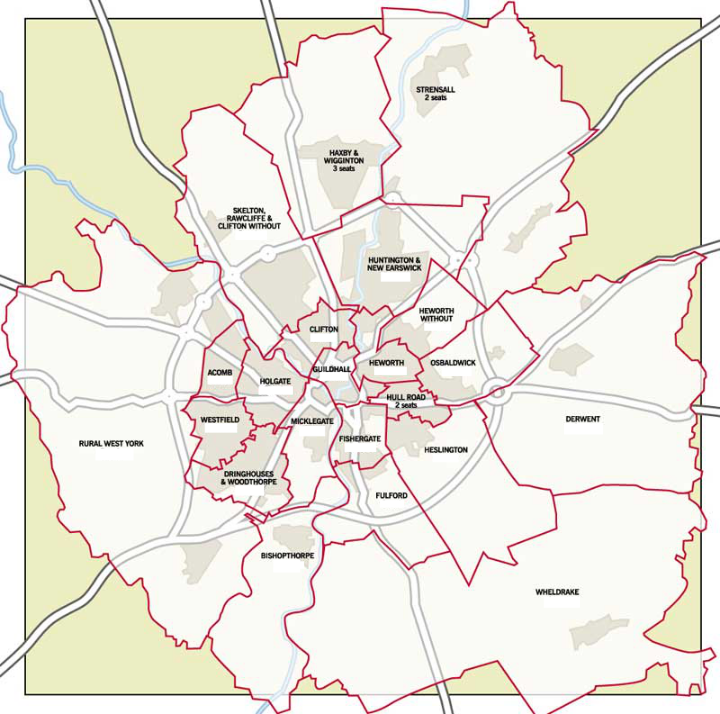
\includegraphics[scale=0.75]{yorkmap.jpg}
\end{figure}
\newpage
\end{document}